\documentclass[12pt]{article}
\usepackage{amsmath}
\usepackage{graphicx}
\usepackage{hyperref}
\usepackage[utf8]{inputenc}
\usepackage{geometry}
\usepackage{mathtools}
\usepackage{empheq}
\usepackage{listings}
\usepackage{xcolor}
\usepackage{minted}
\usepackage{svg}


\definecolor{LightGray}{gray}{0.9}

\graphicspath{ {./assets/} }
\geometry{margin=0.6in}

\title{CHEN 461 HW 6}
\author{Mark Levchenko}
\date{January 2023}

\begin{document}


\begin{enumerate}

%%%%%%%%%%%%%%%%%%%%%%%%%%%%%%%%%%%%%%%%%%%%%%%%%%%%%%%%%%%%%%%%%%%%%%%%
% Problem 1 %%%%%%%%%%%%%%%%%%%%%%%%%%%%%%%%%%%%%%%%%%%%%%%%%%%%%%%%%%%%
%%%%%%%%%%%%%%%%%%%%%%%%%%%%%%%%%%%%%%%%%%%%%%%%%%%%%%%%%%%%%%%%%%%%%%%%
\newpage
    \item Problem 8.1
    
    \[
        G(s) = \frac{s (s + 1)}{s^2 + 4s + 4}  
    \]

    \begin{enumerate}
        \item 
        \begin{align*}
            G(s) &= \frac{s (s + 1)}{(s + 2)^2} \\
            \intertext{Poles}
            (s + 2)^2 &= 0 \\
            \Aboxed{\text{poles} &= -2 \text{ (double)}} \\
            \intertext{Zeros}
            s (s + 1) &= 0 \\
            \Aboxed{\text{zeros} &= 0, -1} \\
            \intertext{Static gain}
            G(0) &= \frac{0 \cdot (0 + 1)}{(0 + 2)^2} \\
            G(0) &= 0 \\
            \Aboxed{k &= 0}
        \end{align*}

        The numerator and denominator are both second order polynomials, and so the relative order is $2-2=0$.

        $\boxed{r=0}$

        The poles of the transfer function are negative, and thus the system is BIBO stable.

        \item 
        \begin{align*}
            Y(s) &= \frac{s (s + 1)}{s^2 + 4s + 4} U(s) \\
            \mathcal{L}^{-1} \left\{s^2 Y(s) + 4s Y(s) + 4 Y(s)\right\} &= \mathcal{L}^{-1} \left\{s^2 U(s) + s U(s)\right\} \\
            \Aboxed{\frac{d^2y}{dt^2} + 4 \frac{dy}{dt} + 4y &= \frac{d^2u}{dt^2} + \frac{du}{dt}}
        \end{align*}

        \item 
        \begin{align*}
            U(s) &= \frac{1}{s} \\
            Y(s) &= \frac{s + 1}{(s + 2)^2} \\
            \mathcal{L}^{-1} \left\{Y(s)\right\} &= \mathcal{L}^{-1} \left\{\frac{s + 2}{(s + 2)^2} - \frac{1}{(s + 2)^2}\right\} \\
            y(t) &= e^{-2t} - t e^{-2t} \\
            \Aboxed{y(t) &= (1 - t) e^{-2t}}
        \end{align*}

        Response Plot:

        \begin{center}
            \includesvg[width=0.8\textwidth]{assets/8.1a.svg}
        \end{center}

        The initial value is 1, and the final value is zero. The numerator of the transfer function is slower than the denominator, and so the response decreases at first. Both the numerator and the denominator are polynomials of the same degree, and so as t approaches infinity, the response goes to zero becasue the numerator is faster than the denominator. 

        \item 
        \begin{align*}
            \intertext{Asymptotic response}
            y(t) &= \frac{dG}{ds}(0) + G(0) \\
            \frac{dG}{ds}(0) &= 0.25 \\
            G(0) &= 0 \\
            \Aboxed{y(t) &= 0.25} 
        \end{align*}

        \item 
        \begin{align*}
            G(i\omega) &= \frac{i\omega (i\omega + 1)}{(i\omega)^2 + 4i\omega + 4} \\
            G(i\omega) &= \frac{-\omega^2 + i\omega}{(4 - \omega^2) + 4i\omega} \cdot \frac{(4 - \omega^2) - 4i\omega}{(4 - \omega^2) - 4i\omega} \\ 
            G(i\omega) &= \frac{-\omega^2 (4 - \omega^2) + 4i\omega^3 + i\omega (4 - \omega^2) + 4\omega^2}{(4 - \omega^2) - (4\omega)^2} \\
            G(i\omega) &= \frac{\omega^4 + (4\omega + 3\omega^3) i}{\omega^4 + 8\omega^2 + 16} \\
            G(i\omega) &= \frac{\omega^4 + (4\omega + 3\omega^3) i}{\left(\omega^2 + 4\right)^2} \\
            \intertext{Separate real and imaginary parts}
            \text{Re} \left\{G(i\omega)\right\} &= \frac{\omega^4}{\left(\omega^2 + 4\right)^2} \\
            \text{Im} \left\{G(i\omega)\right\} &= \frac{4\omega + 3\omega^3}{\left(\omega^2 + 4\right)^2} \\
            \intertext{Asymptotic response}
            \Aboxed{y(t) &= \frac{\omega^4}{\left(\omega^2 + 4\right)^2} \sin\left(\omega t\right) + \frac{4\omega + 3\omega^3}{\left(\omega^2 + 4\right)^2} \cos\left(\omega t\right)}
        \end{align*}

        \item Verify answers to parts c through e by simulating an input to the system. LTI system will be created in code using the transfer function numerator and denominator.
        
        Verify step response:

        \begin{center}
            \includesvg[width=0.8\textwidth]{assets/p1f_step.svg}
        \end{center}

        Analytical and simulated plots line up perfectly.

        Verify ramp response asymptote:

        \begin{center}
            \includesvg[width=0.8\textwidth]{assets/p1f_ramp.svg}
        \end{center}

        Response goes to 0.25 as t goes to infinity just as predicted.

        Verify sinusoidal response:

        \begin{center}
            \includesvg[width=0.8\textwidth]{assets/p1f_sin.svg}
        \end{center}

        For large t, the analytical response lines up perfectly with the simulated response.
    \end{enumerate}
    
    Code for analytical solution verification:

\begin{minted}[
framesep=2mm,
baselinestretch=1.2,
bgcolor=LightGray,
fontsize=\footnotesize,
breaklines,
]{python}
import numpy as np
import matplotlib.pyplot as plt
from scipy import signal

# LTI system
sys = signal.lti([1, 1, 0], [1, 4, 4])

# Step response
t_step, y_step = signal.step(sys)
step_analytical = lambda t: (1 - t) * np.exp(-2 * t)

plt.plot(t_step, y_step, label="Simulated Response")
plt.plot(t_step, step_analytical(t_step), "--", label="Analytical Response")
plt.xlabel(r"$t$")
plt.ylabel(r"$y(t)$")
plt.title("Problem 8.1 Verify Analytical Step Response")
plt.legend(); plt.show()

# Ramp response
t_ramp = np.linspace(0, 10, 100)
t_ramp, y_ramp, _ = signal.lsim(sys, t_ramp, t_ramp)

plt.plot(t_ramp, y_ramp, label="Simulated Response")
plt.xlabel(r"$t$")
plt.ylabel(r"$y(t)$")
plt.title("Problem 8.1 Verify Analytical Ramp Response")
plt.legend()
plt.show()

# Sinusoidal response for omega=1
sin_analytical = lambda t: np.sin(t) / 25 + np.cos(t) * 7 / 25
t_sin = np.linspace(0, 20, 100)
u_sin  = np.sin(t_sin)
t_sin, y_sin, _ = signal.lsim(sys, u_sin, t_sin)

plt.plot(t_sin, y_sin, label="Simulated Response")
plt.plot(t_sin, sin_analytical(t_sin), '--', label="Analytical Response")
plt.xlabel(r"$t$")
plt.ylabel(r"$y(t)$")
plt.title("Problem 8.1 Verify Analytical Sinusoidal Response")
plt.legend()
plt.show()
\end{minted}
    
%%%%%%%%%%%%%%%%%%%%%%%%%%%%%%%%%%%%%%%%%%%%%%%%%%%%%%%%%%%%%%%%%%%%%%%%
% Problem 2 %%%%%%%%%%%%%%%%%%%%%%%%%%%%%%%%%%%%%%%%%%%%%%%%%%%%%%%%%%%%
%%%%%%%%%%%%%%%%%%%%%%%%%%%%%%%%%%%%%%%%%%%%%%%%%%%%%%%%%%%%%%%%%%%%%%%%
\newpage
    \item Problem 8.10
    \begin{enumerate}
        \item 
        \begin{align*}
            A &= \begin{bmatrix}
                1 & 0 \\
                1 & -1 \\
            \end{bmatrix} \\
            B &= \begin{bmatrix}
                0 \\
                1 \\
            \end{bmatrix} \\
            C &= \begin{bmatrix}
                1 & 1 \\
            \end{bmatrix} \\
            D &= 0 \\    
            G(s) &= C (s I - A)^{-1} B + D \\
            G(s) &= \begin{bmatrix}
                1 & 1 \\
            \end{bmatrix}
            \left(
                \begin{bmatrix}
                    s & 0 \\
                    0 & s \\
                \end{bmatrix} - 
                \begin{bmatrix}
                    1 & 0 \\
                    1 & -1 \\
                \end{bmatrix}
            \right)^{-1}
            \begin{bmatrix}
                0 \\
                1 \\
            \end{bmatrix} \\
            G(s) &= \frac{1}{s + 1} \\
            \text{degree of numerator} &= 0 \\
            \text{degree of denominator} &= 1 \\
            \text{relative order} &= 1 - 0 \\
            \Aboxed{\text{relative order} &= 1}
        \end{align*}

        \item 
        \begin{align*}
            0 &= \mathrm{det} \begin{bmatrix}
                \lambda - 1 & 0 \\
                1 & \lambda + 1 \\
            \end{bmatrix} \\
            0 &= (\lambda - 1) (\lambda + 1) \\
            \lambda &= 1, -1
        \end{align*}

        The system is not asymptotically stable. One of the eigenvalues is positive.

        \item 
        \begin{align*}
            \intertext{From part A}
            \Aboxed{G(s) &= \frac{1}{s + 1}} \\
            \intertext{Poles}
            s + 1 &= 0 \\
            \Aboxed{\text{poles} &= -1} \\
            \Aboxed{\text{zeros} &= \text{none}} \\
        \end{align*}

        \item The system is BIBO stable becasue the poles are negative.
    \end{enumerate}
    
%%%%%%%%%%%%%%%%%%%%%%%%%%%%%%%%%%%%%%%%%%%%%%%%%%%%%%%%%%%%%%%%%%%%%%%%
% Problem 3 %%%%%%%%%%%%%%%%%%%%%%%%%%%%%%%%%%%%%%%%%%%%%%%%%%%%%%%%%%%%
%%%%%%%%%%%%%%%%%%%%%%%%%%%%%%%%%%%%%%%%%%%%%%%%%%%%%%%%%%%%%%%%%%%%%%%%
\newpage
    \item Problem 9.3
    
    (i)

    \begin{align*}
        G(s) &= \frac{1}{s} \cdot \frac{1}{\frac{s}{10} + 1} \cdot \frac{1}{10s + 1} \\
        \intertext{$\frac{1}{s}$ magnitube and phase angle}
        \text{AR} &= \frac{1}{\omega} \\
        \phi &= -90^\circ \\
        \intertext{$\frac{1}{\frac{s}{10} + 1}$ magnitube and phase angle}
        \text{AR} &= \frac{1}{\sqrt{\frac{\omega^2}{100}+1}} \\
        \phi &= -\tan^{-1}\left(\frac{\omega}{10}\right) \\
        \intertext{$\frac{1}{10s + 1}$ magnitube and phase angle}
        \text{AR} &= \frac{1}{\sqrt{100\omega^2+1}} \\
        \phi &= -\tan^{-1}\left(10\omega\right) \\
        \intertext{Overall}
        \text{AR} &= \frac{1}{\omega} \frac{1}{\sqrt{\frac{\omega^2}{100}+1}} \frac{1}{\sqrt{100\omega^2+1}} \\
        \phi &= -90^\circ - \tan^{-1}\left(\frac{\omega}{10}\right) - \tan^{-1}\left(10\omega\right) \\
    \end{align*}

    Sketch bode plots:

    \begin{center}
        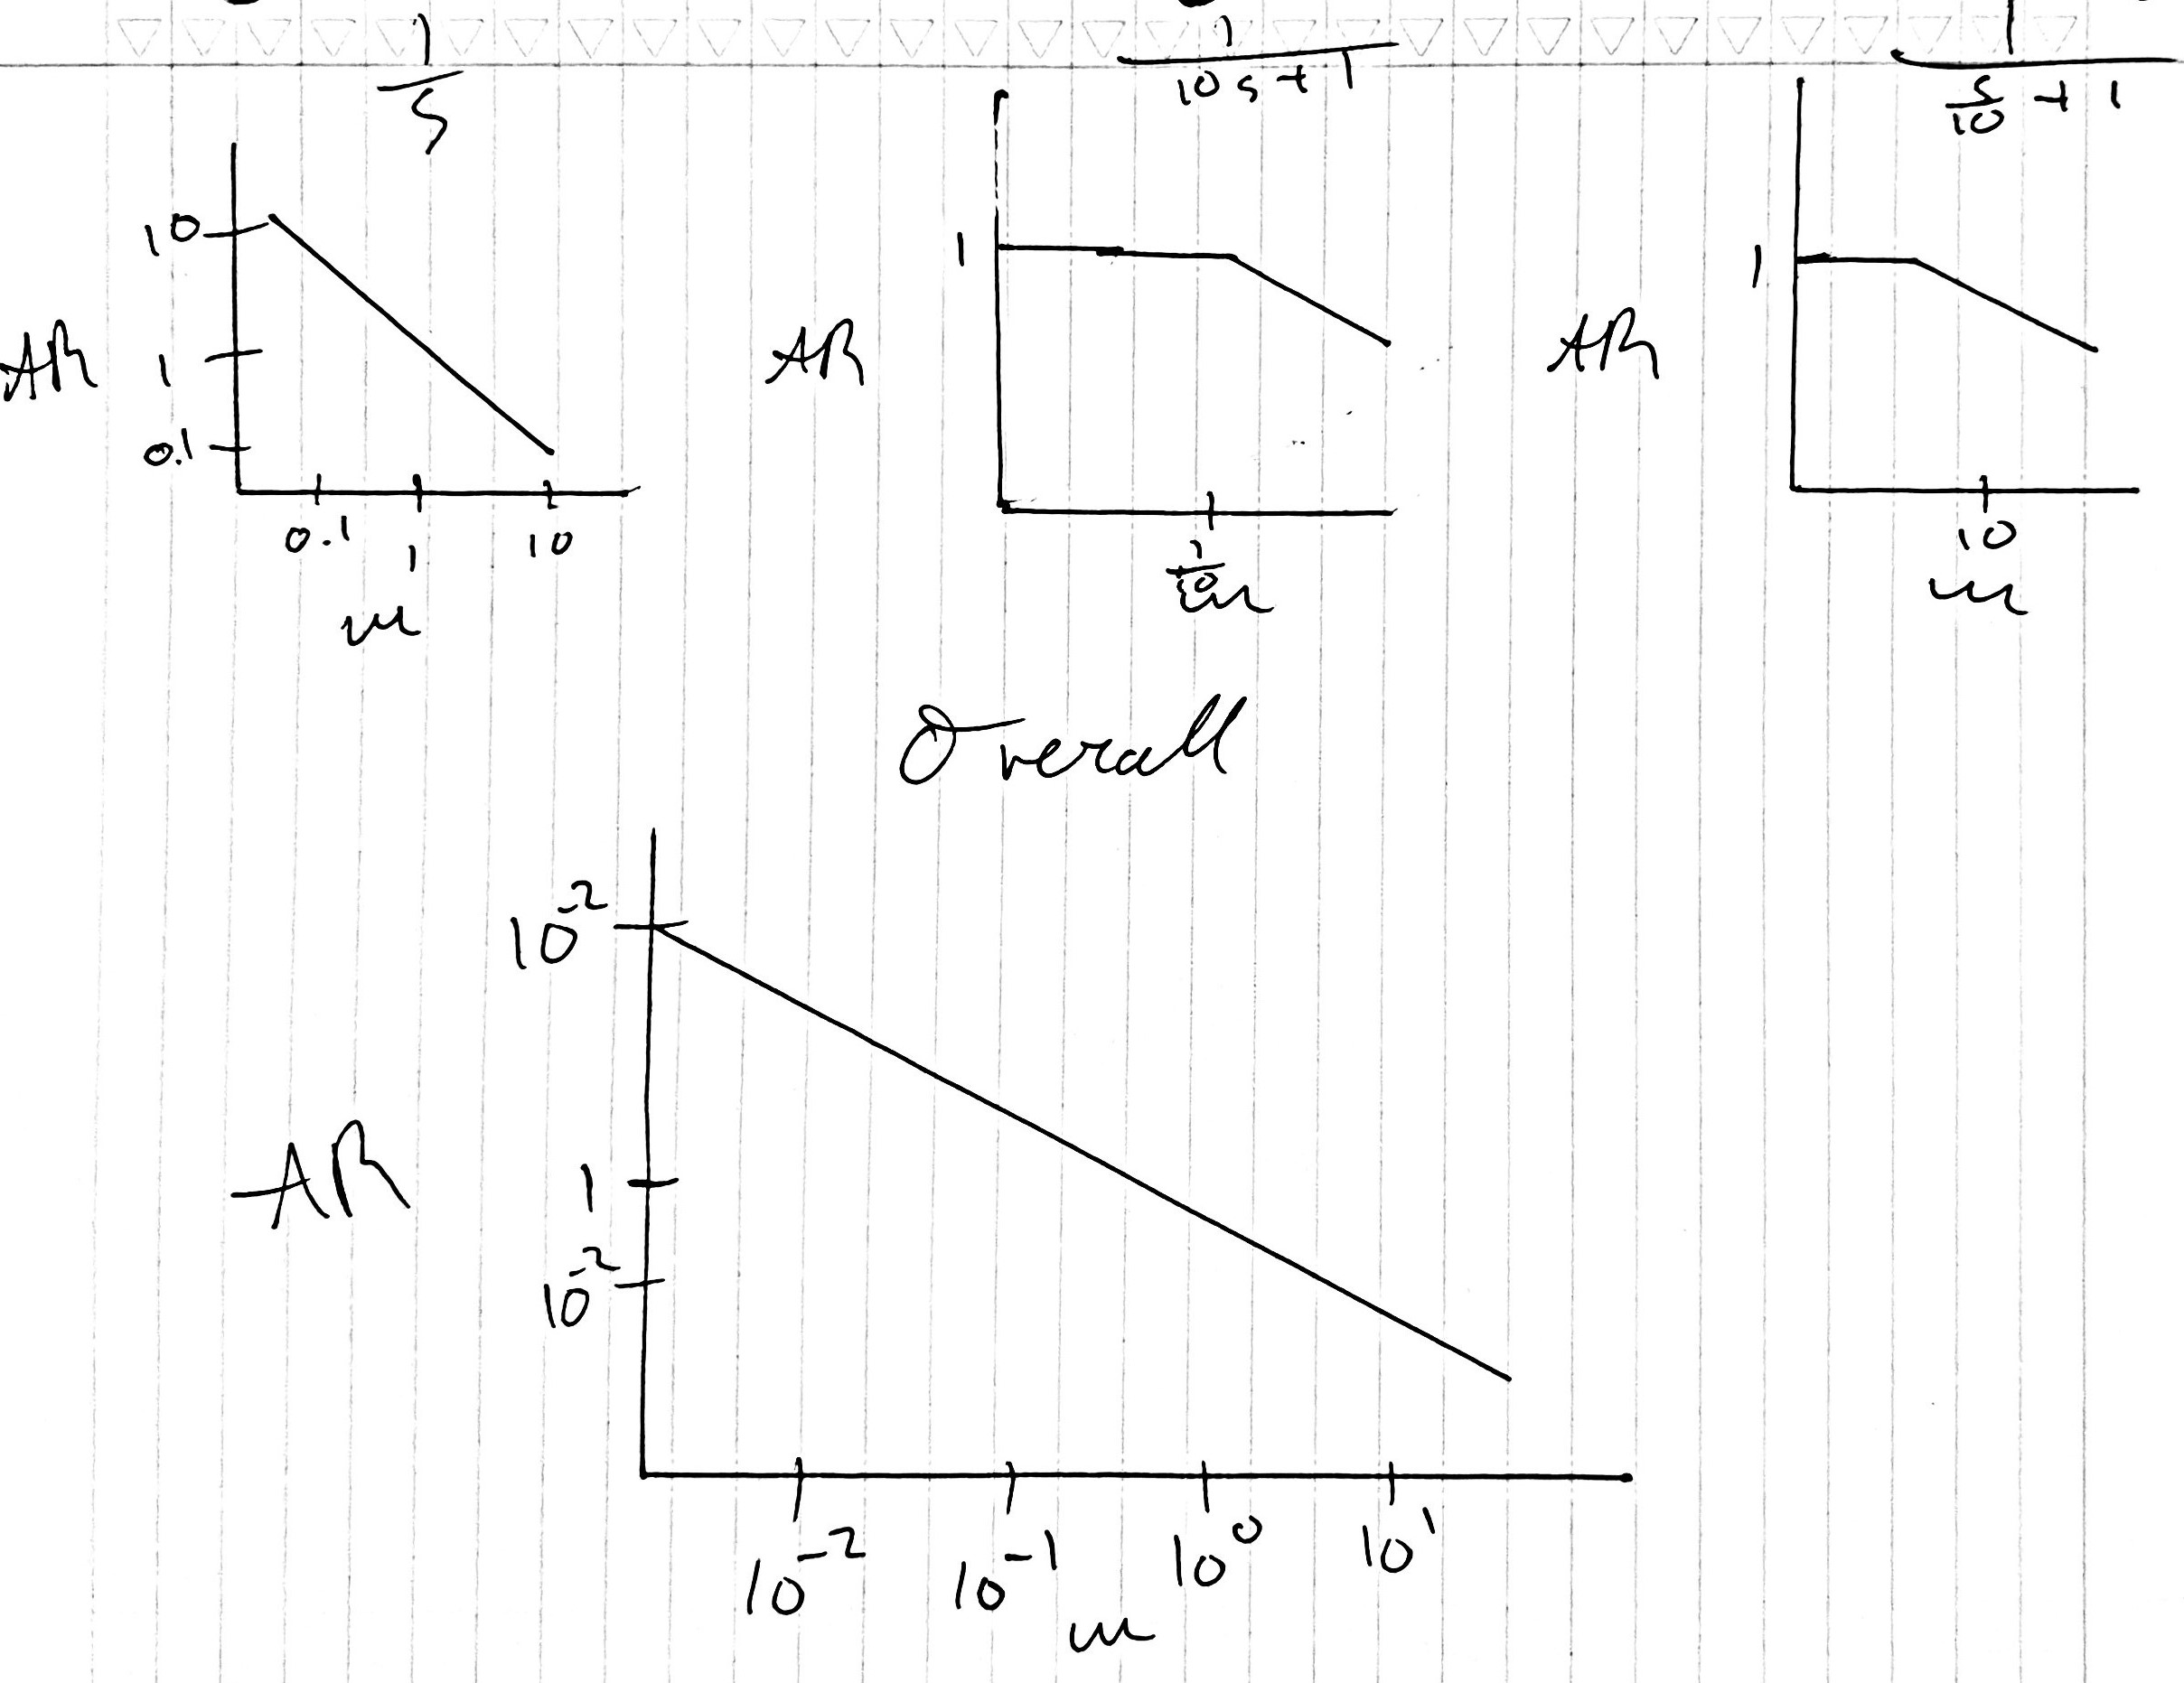
\includegraphics[width=0.8\textwidth]{assets/i_mag.jpg}
        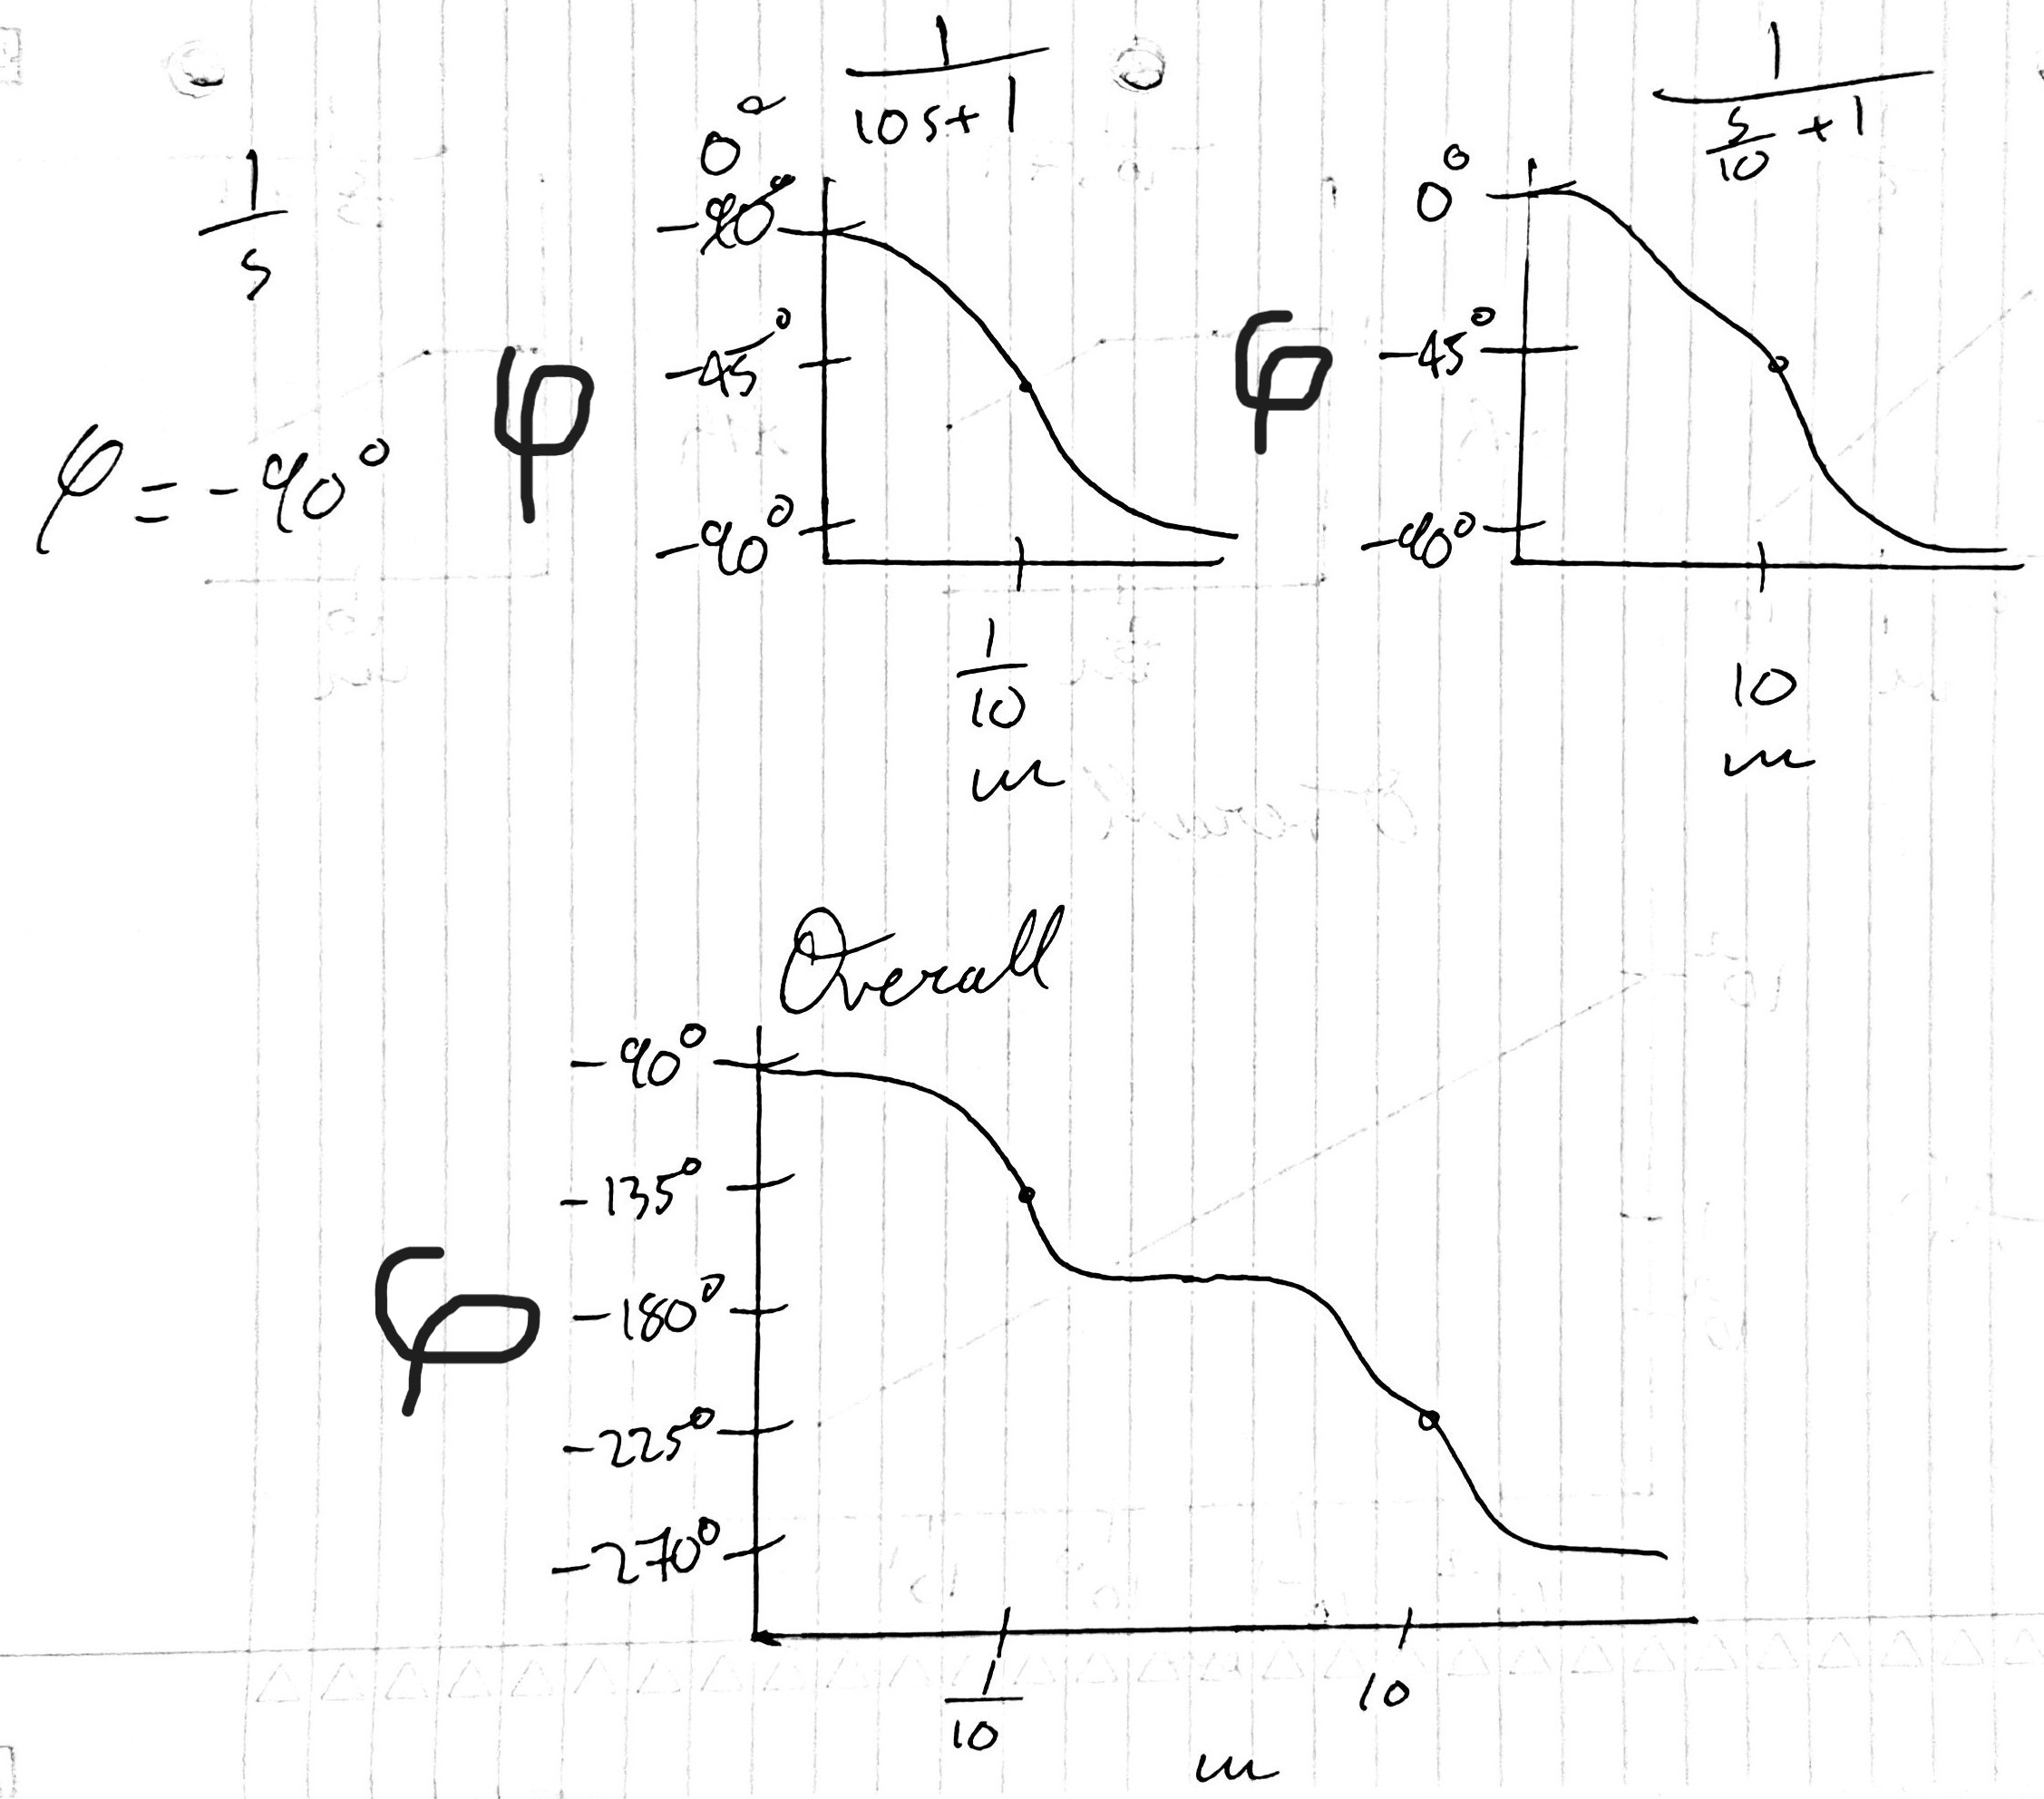
\includegraphics[width=0.8\textwidth]{assets/i_phase.jpg}
    \end{center}

    Verify:

    \begin{center}
        \includesvg[width=0.8\textwidth]{assets/p3_i.svg}
    \end{center}

    (ii)

    \begin{align*}
        G(s) &= \frac{10s+1}{s^2 + 2s + 1} \\
        \intertext{$10s+1$ magnitube and phase angle}
        \text{AR} &= \sqrt{100\omega^2+1} \\
        \phi &= \tan^{-1}\left(10\omega\right) \\
        \intertext{$\frac{1}{s^2 + 2s + 1}$ magnitube and phase angle}
        \text{AR} &= \frac{1}{\sqrt{\left(1-\omega^2\right)^2 + 4\omega^2}} \\
        \phi &= -\cos^{-1}\left(\frac{1-\omega^2}{\sqrt{\left(1-\omega^2\right)^2 + 4\omega^2}}\right) \\
        \intertext{Overall}
        \text{AR} &= \frac{\sqrt{100\omega^2+1}}{\sqrt{\left(1-\omega^2\right)^2 + 4\omega^2}} \\
        \phi &= \tan^{-1}\left(10\omega\right) - \cos^{-1}\left(\frac{1-\omega^2}{\sqrt{\left(1-\omega^2\right)^2 + 4\omega^2}}\right)\\
    \end{align*}

    Sketch bode plots:

    \begin{center}
        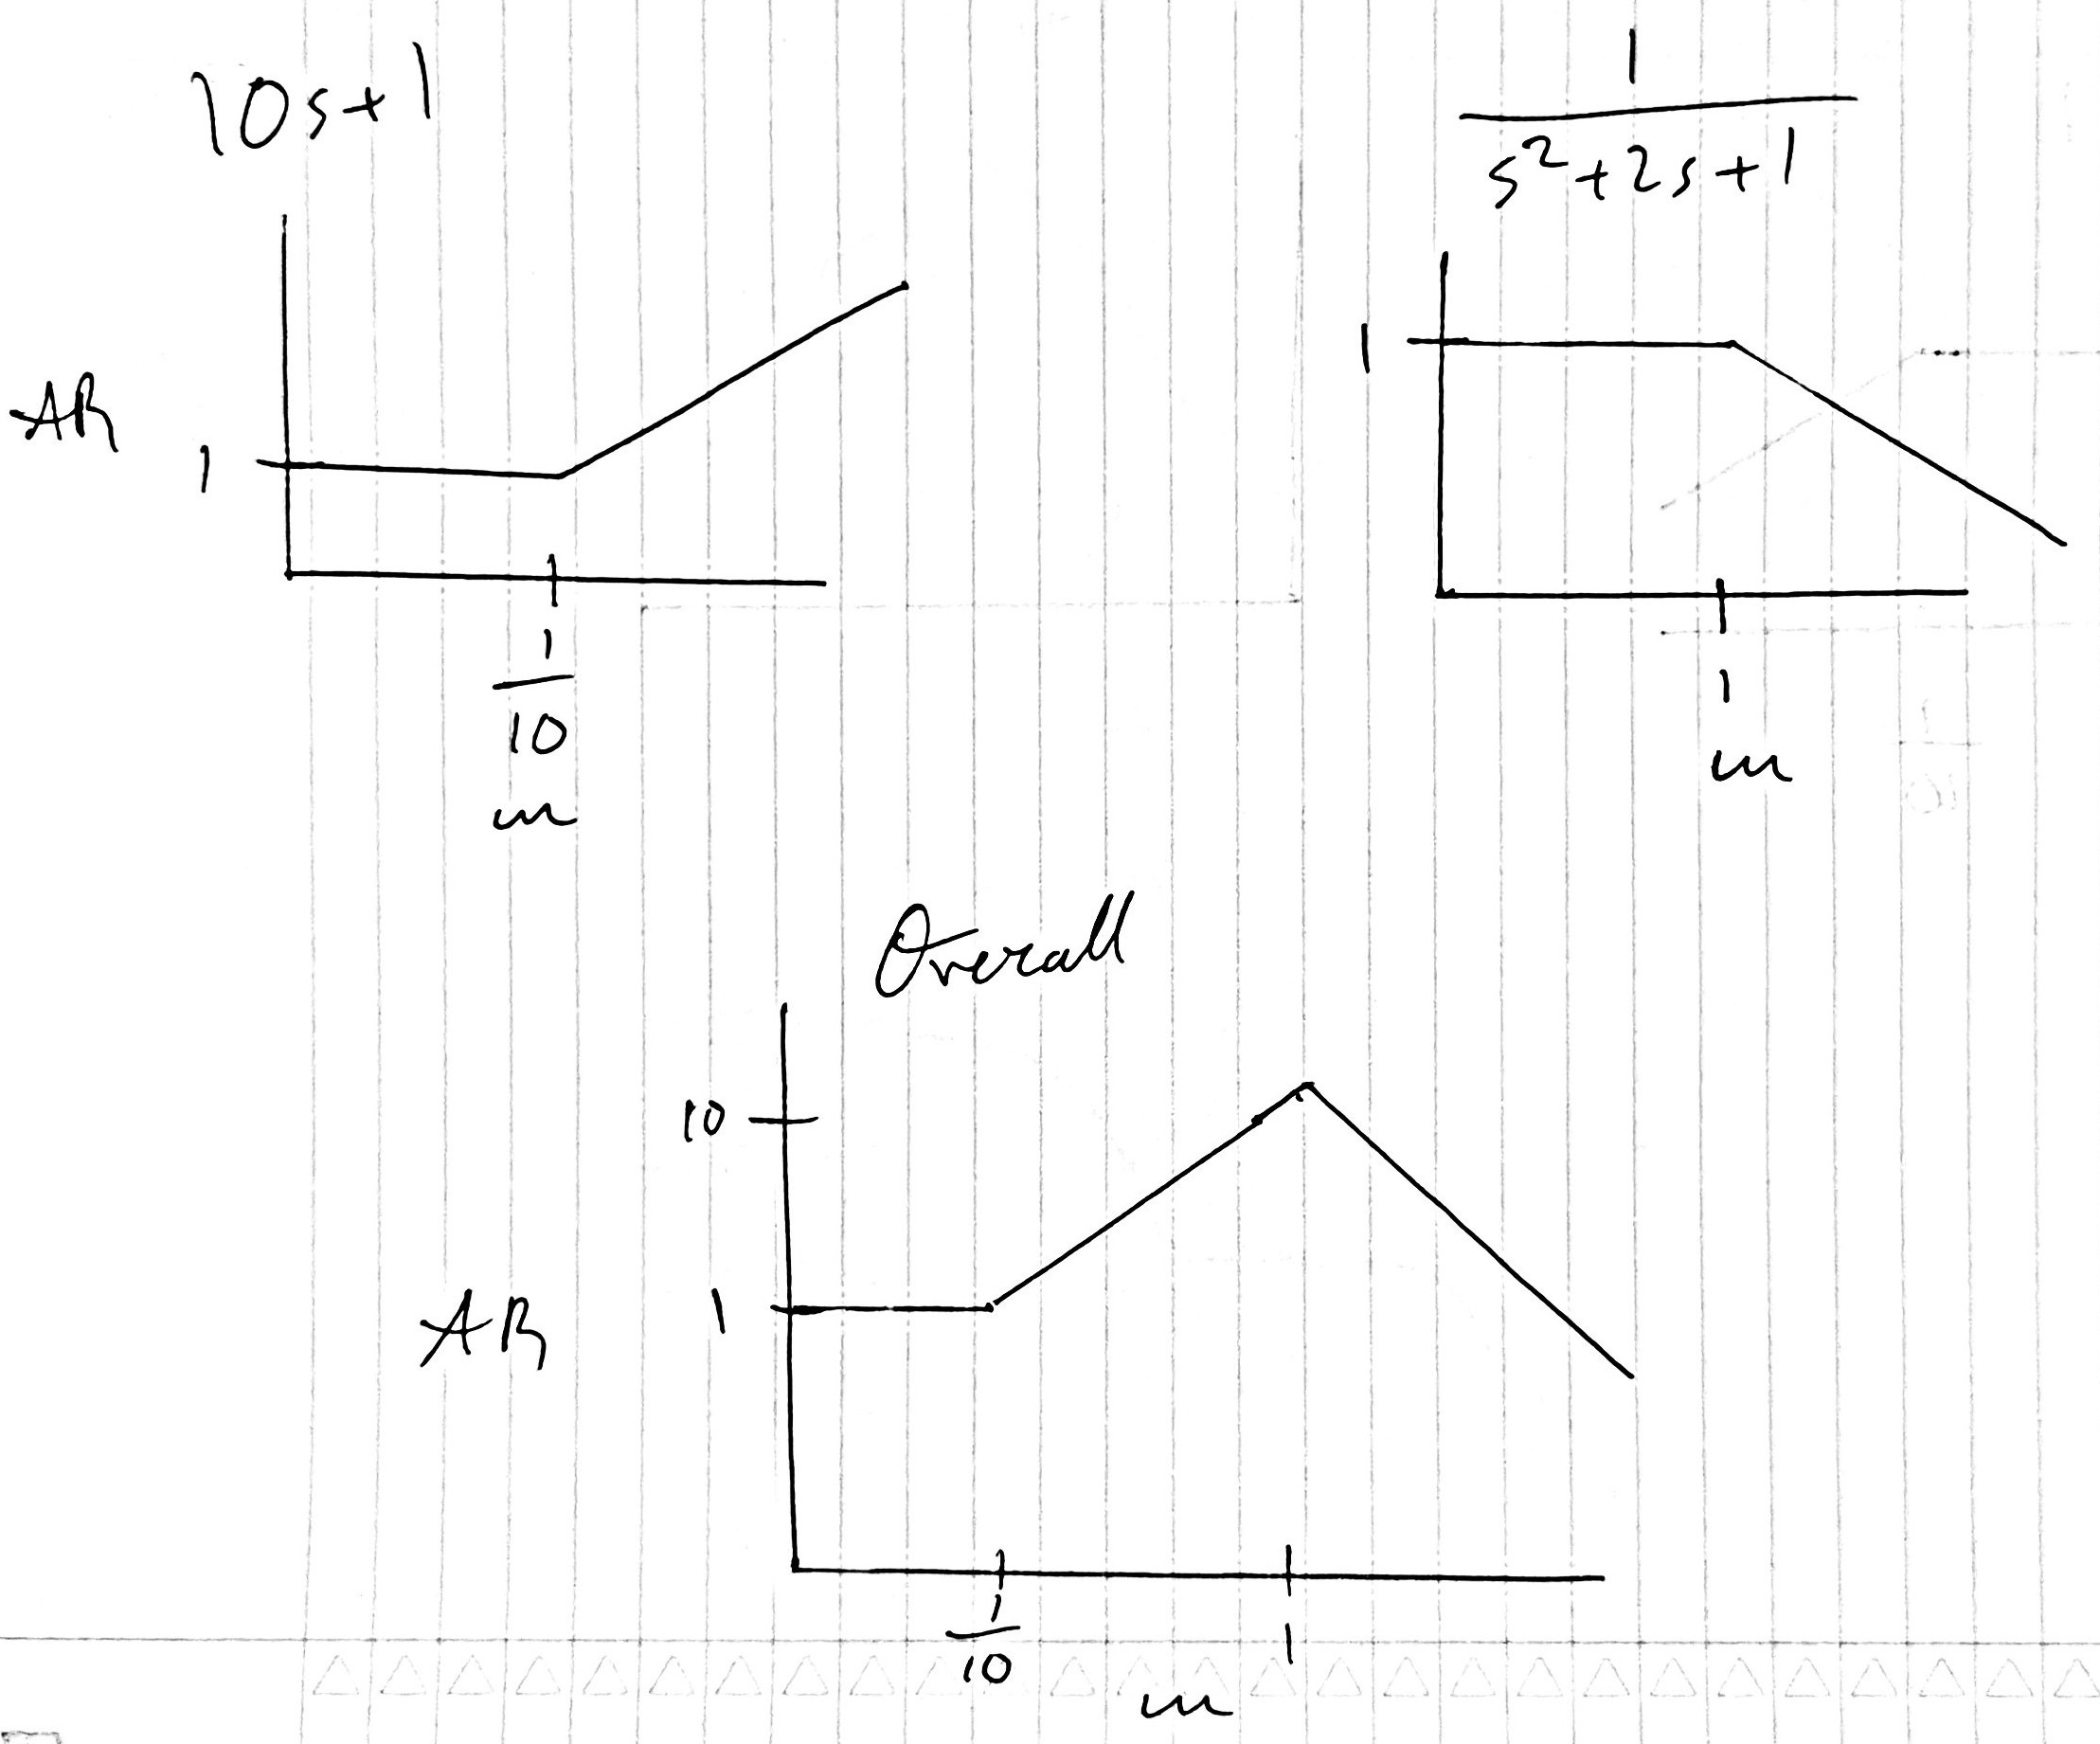
\includegraphics[width=0.8\textwidth]{assets/ii_mag.jpg}
        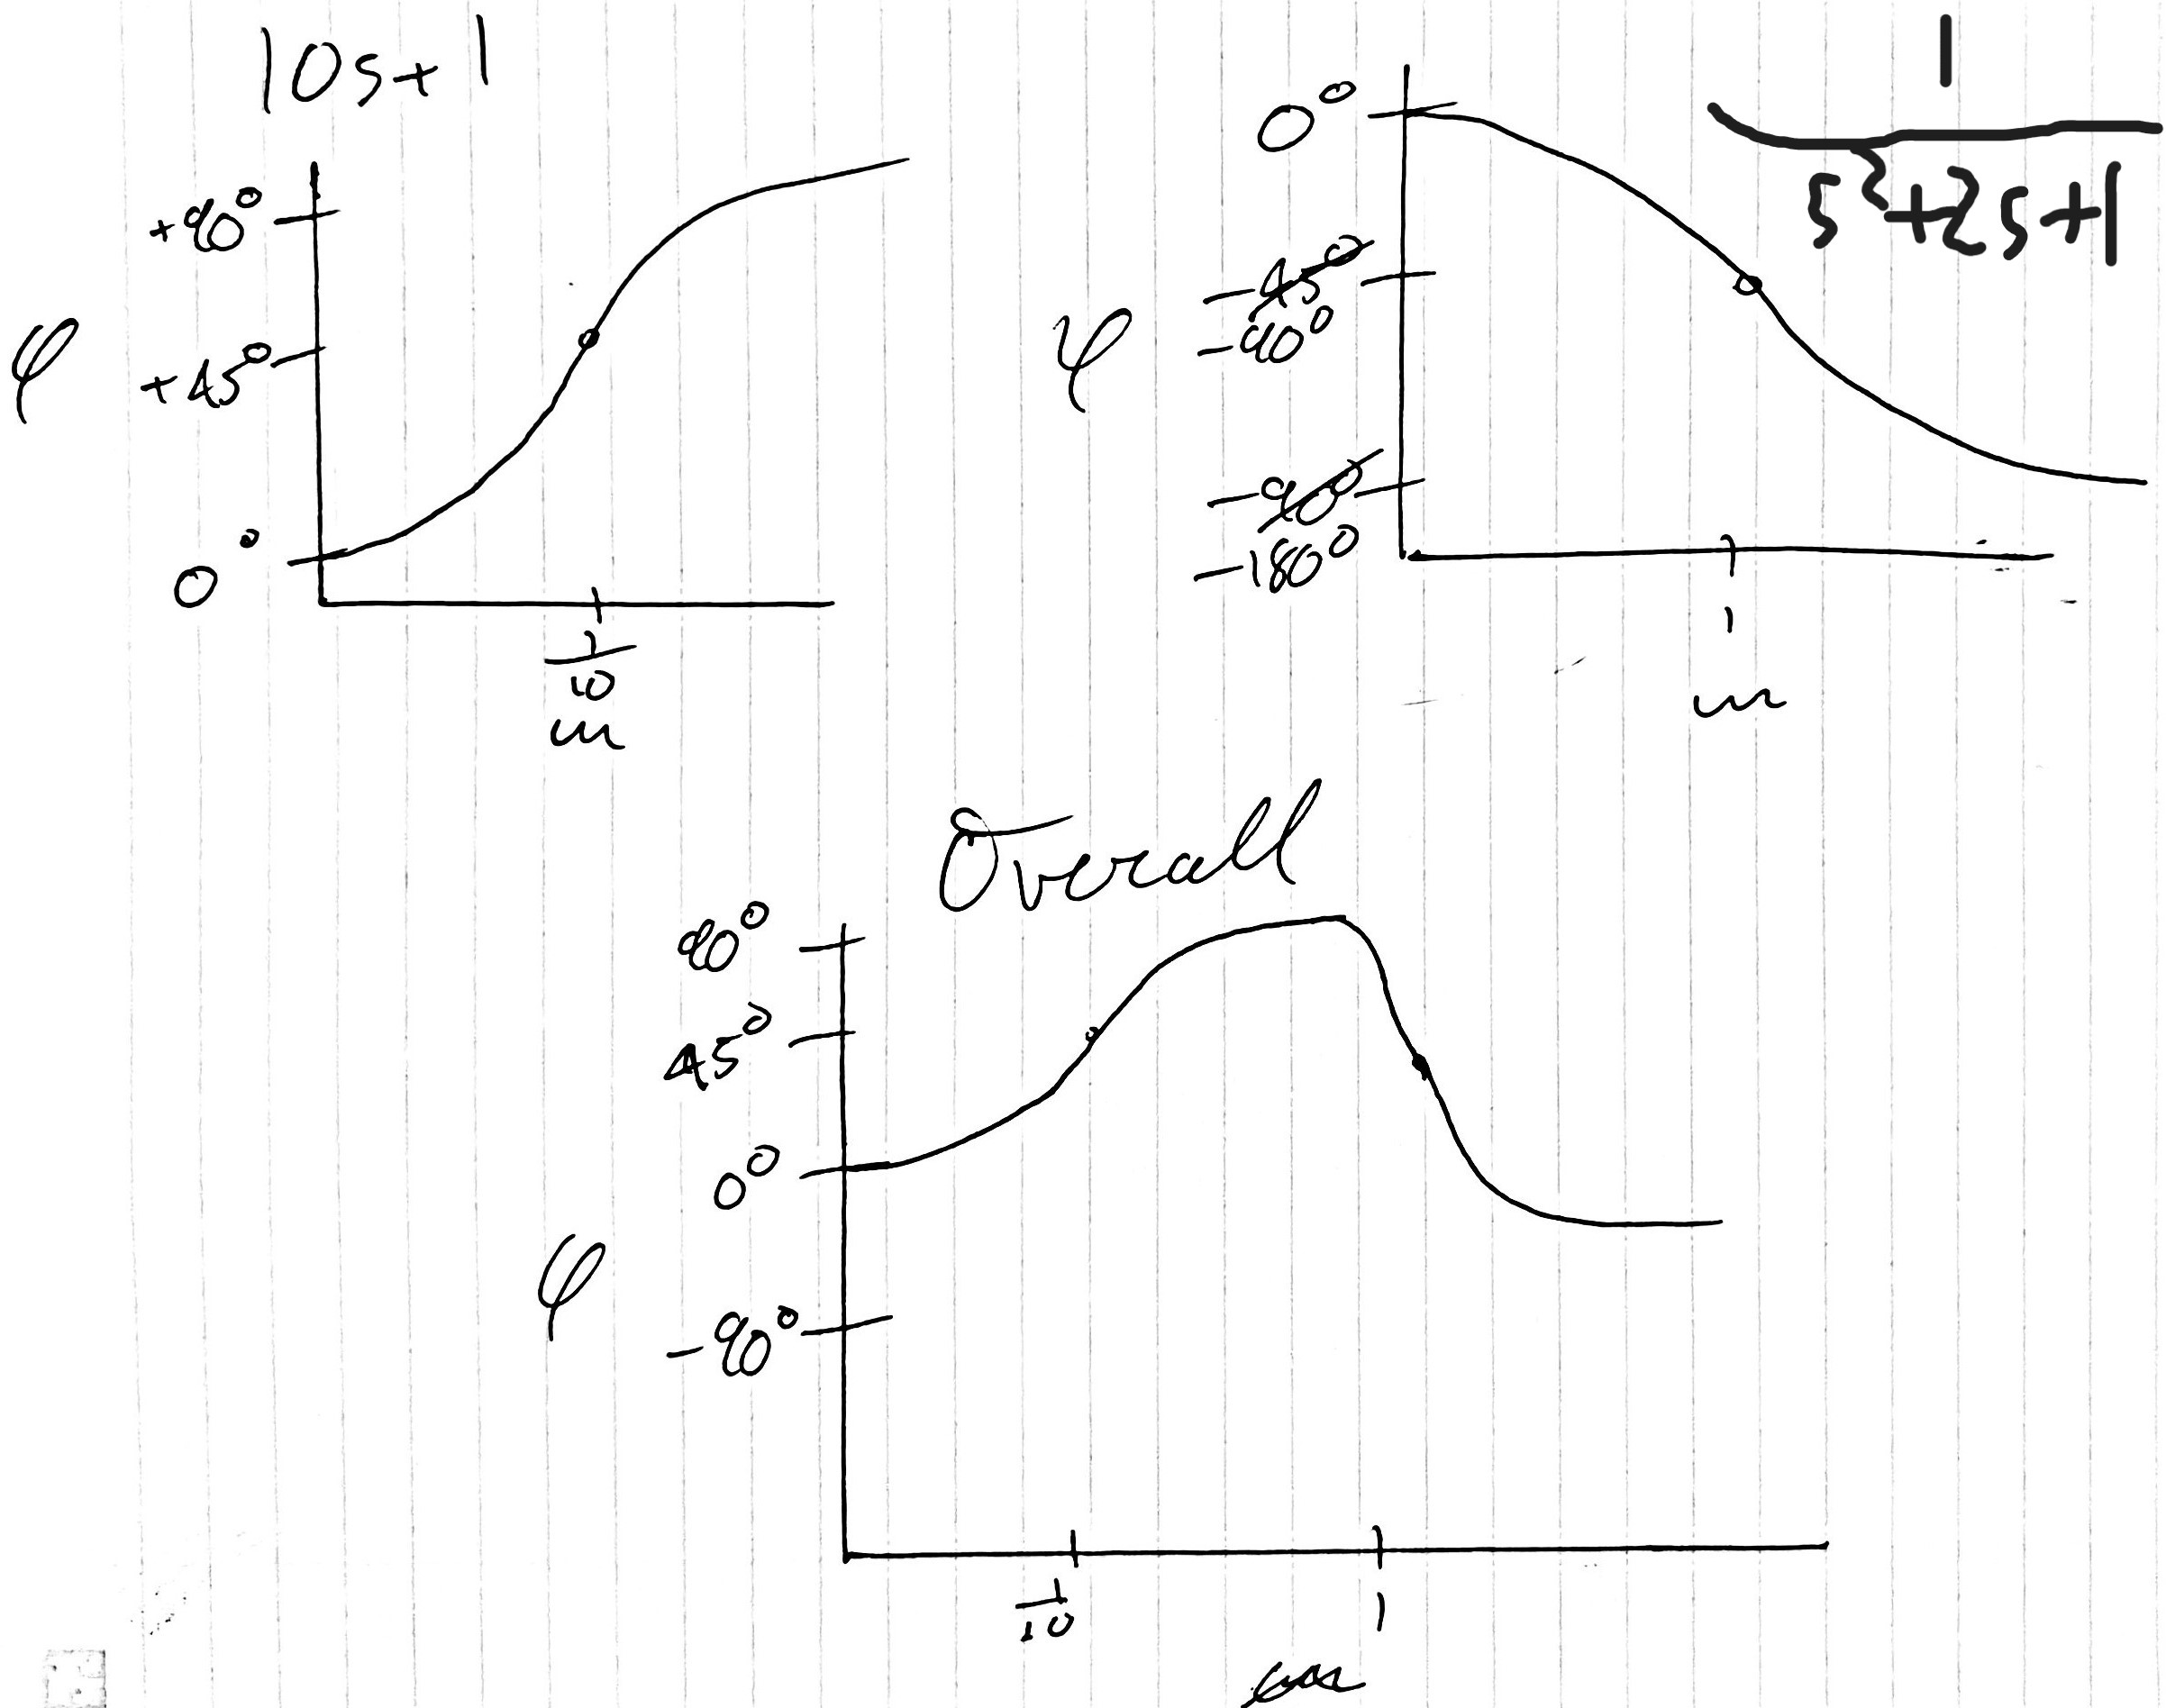
\includegraphics[width=0.8\textwidth]{assets/ii_phase.jpg}
    \end{center}

    Verify:

    \begin{center}
        \includesvg[width=0.8\textwidth]{assets/p3_ii.svg}
    \end{center}

    (iii)

    \begin{align*}
        G(s) &= \frac{1}{s^2 + 2s + 1} \cdot \frac{1-10s}{1+10s} \cdot (10s+1)\\
        \intertext{$10s+1$ magnitube and phase angle}
        \text{AR} &= \sqrt{100\omega^2+1} \\
        \phi &= \tan^{-1}\left(10\omega\right) \\
        \intertext{$\frac{1}{s^2 + 2s + 1}$ magnitube and phase angle}
        \text{AR} &= \frac{1}{\sqrt{\left(1-\omega^2\right)^2 + 4\omega^2}} \\
        \phi &= -\cos^{-1}\left(\frac{1-\omega^2}{\sqrt{\left(1-\omega^2\right)^2 + 4\omega^2}}\right) \\
        \intertext{$\frac{1-10s}{1+10s}$ magnitube and phase angle}
        \text{AR} &= 1 \\
        \phi &= -2\tan^{-1}\left(10\omega\right) \\
        \intertext{Overall}
        \text{AR} &= \frac{\sqrt{100\omega^2+1}}{\sqrt{\left(1-\omega^2\right)^2 + 4\omega^2}} \\
        \phi &= \tan^{-1}\left(10\omega\right) - \cos^{-1}\left(\frac{1-\omega^2}{\sqrt{\left(1-\omega^2\right)^2 + 4\omega^2}}\right) - 2\tan^{-1}\left(10\omega\right) \\
    \end{align*}

    Sketch bode plots:

    \begin{center}
        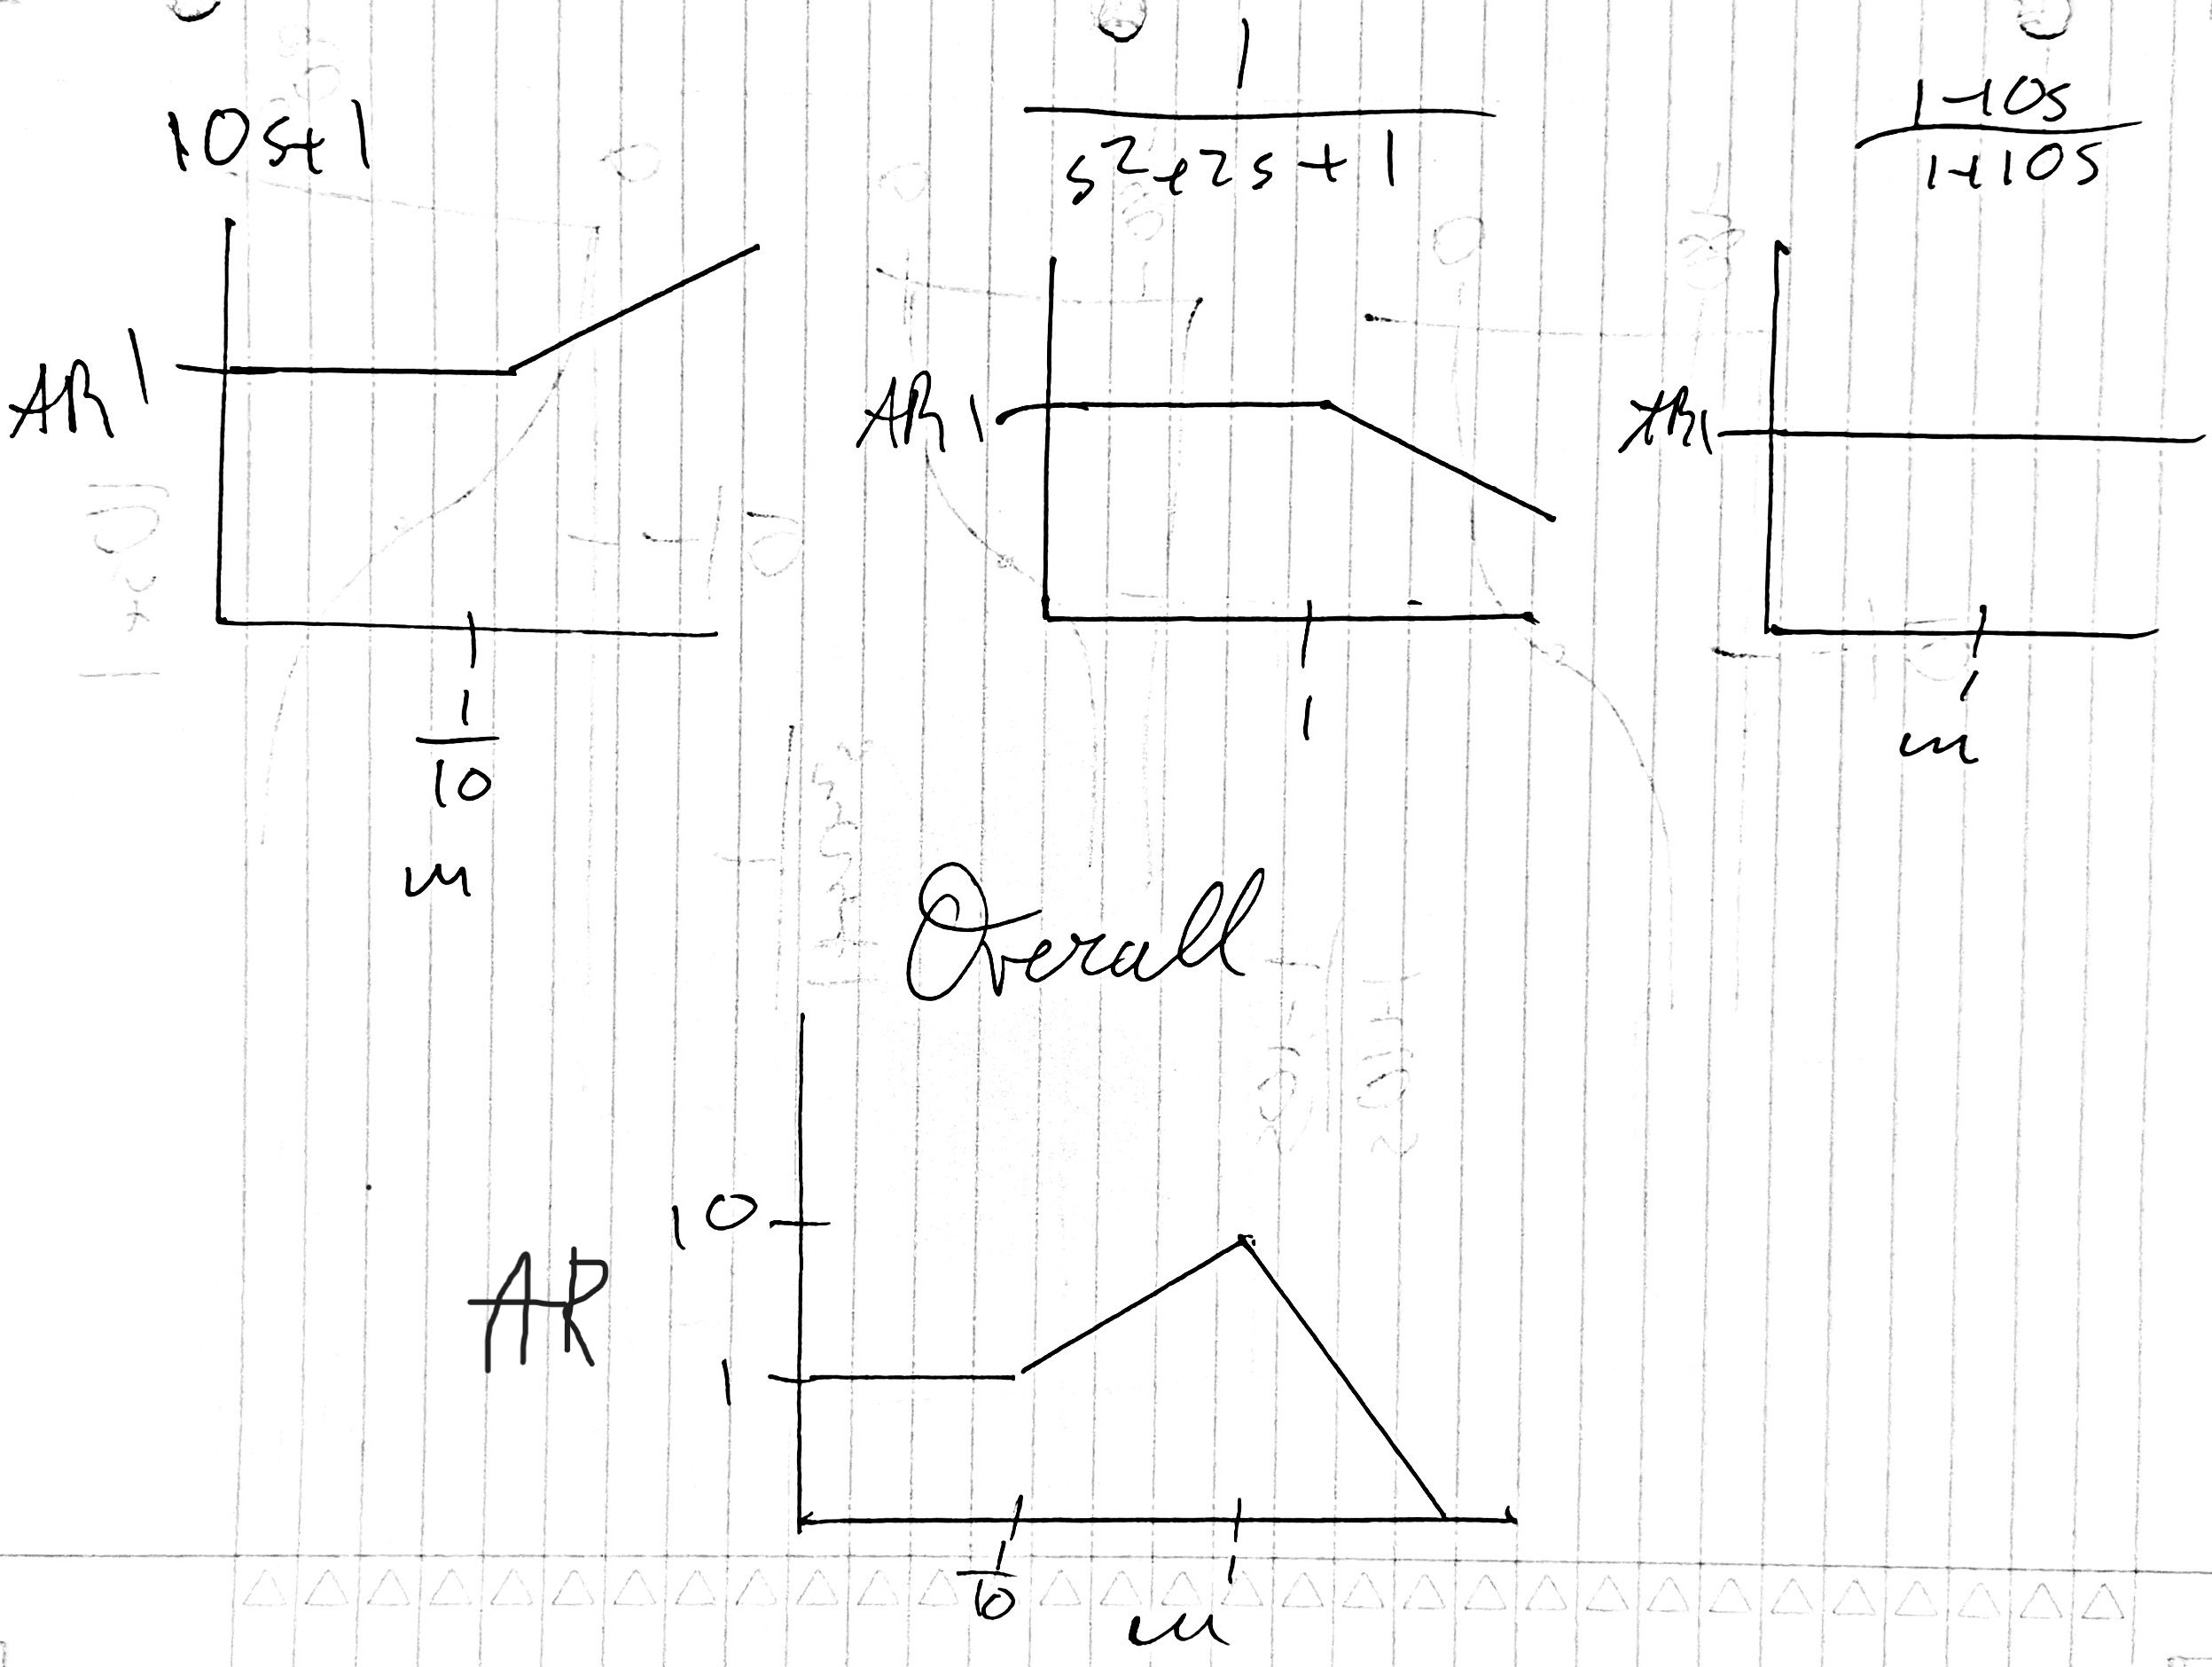
\includegraphics[width=0.8\textwidth]{assets/iii_mag.jpg}
        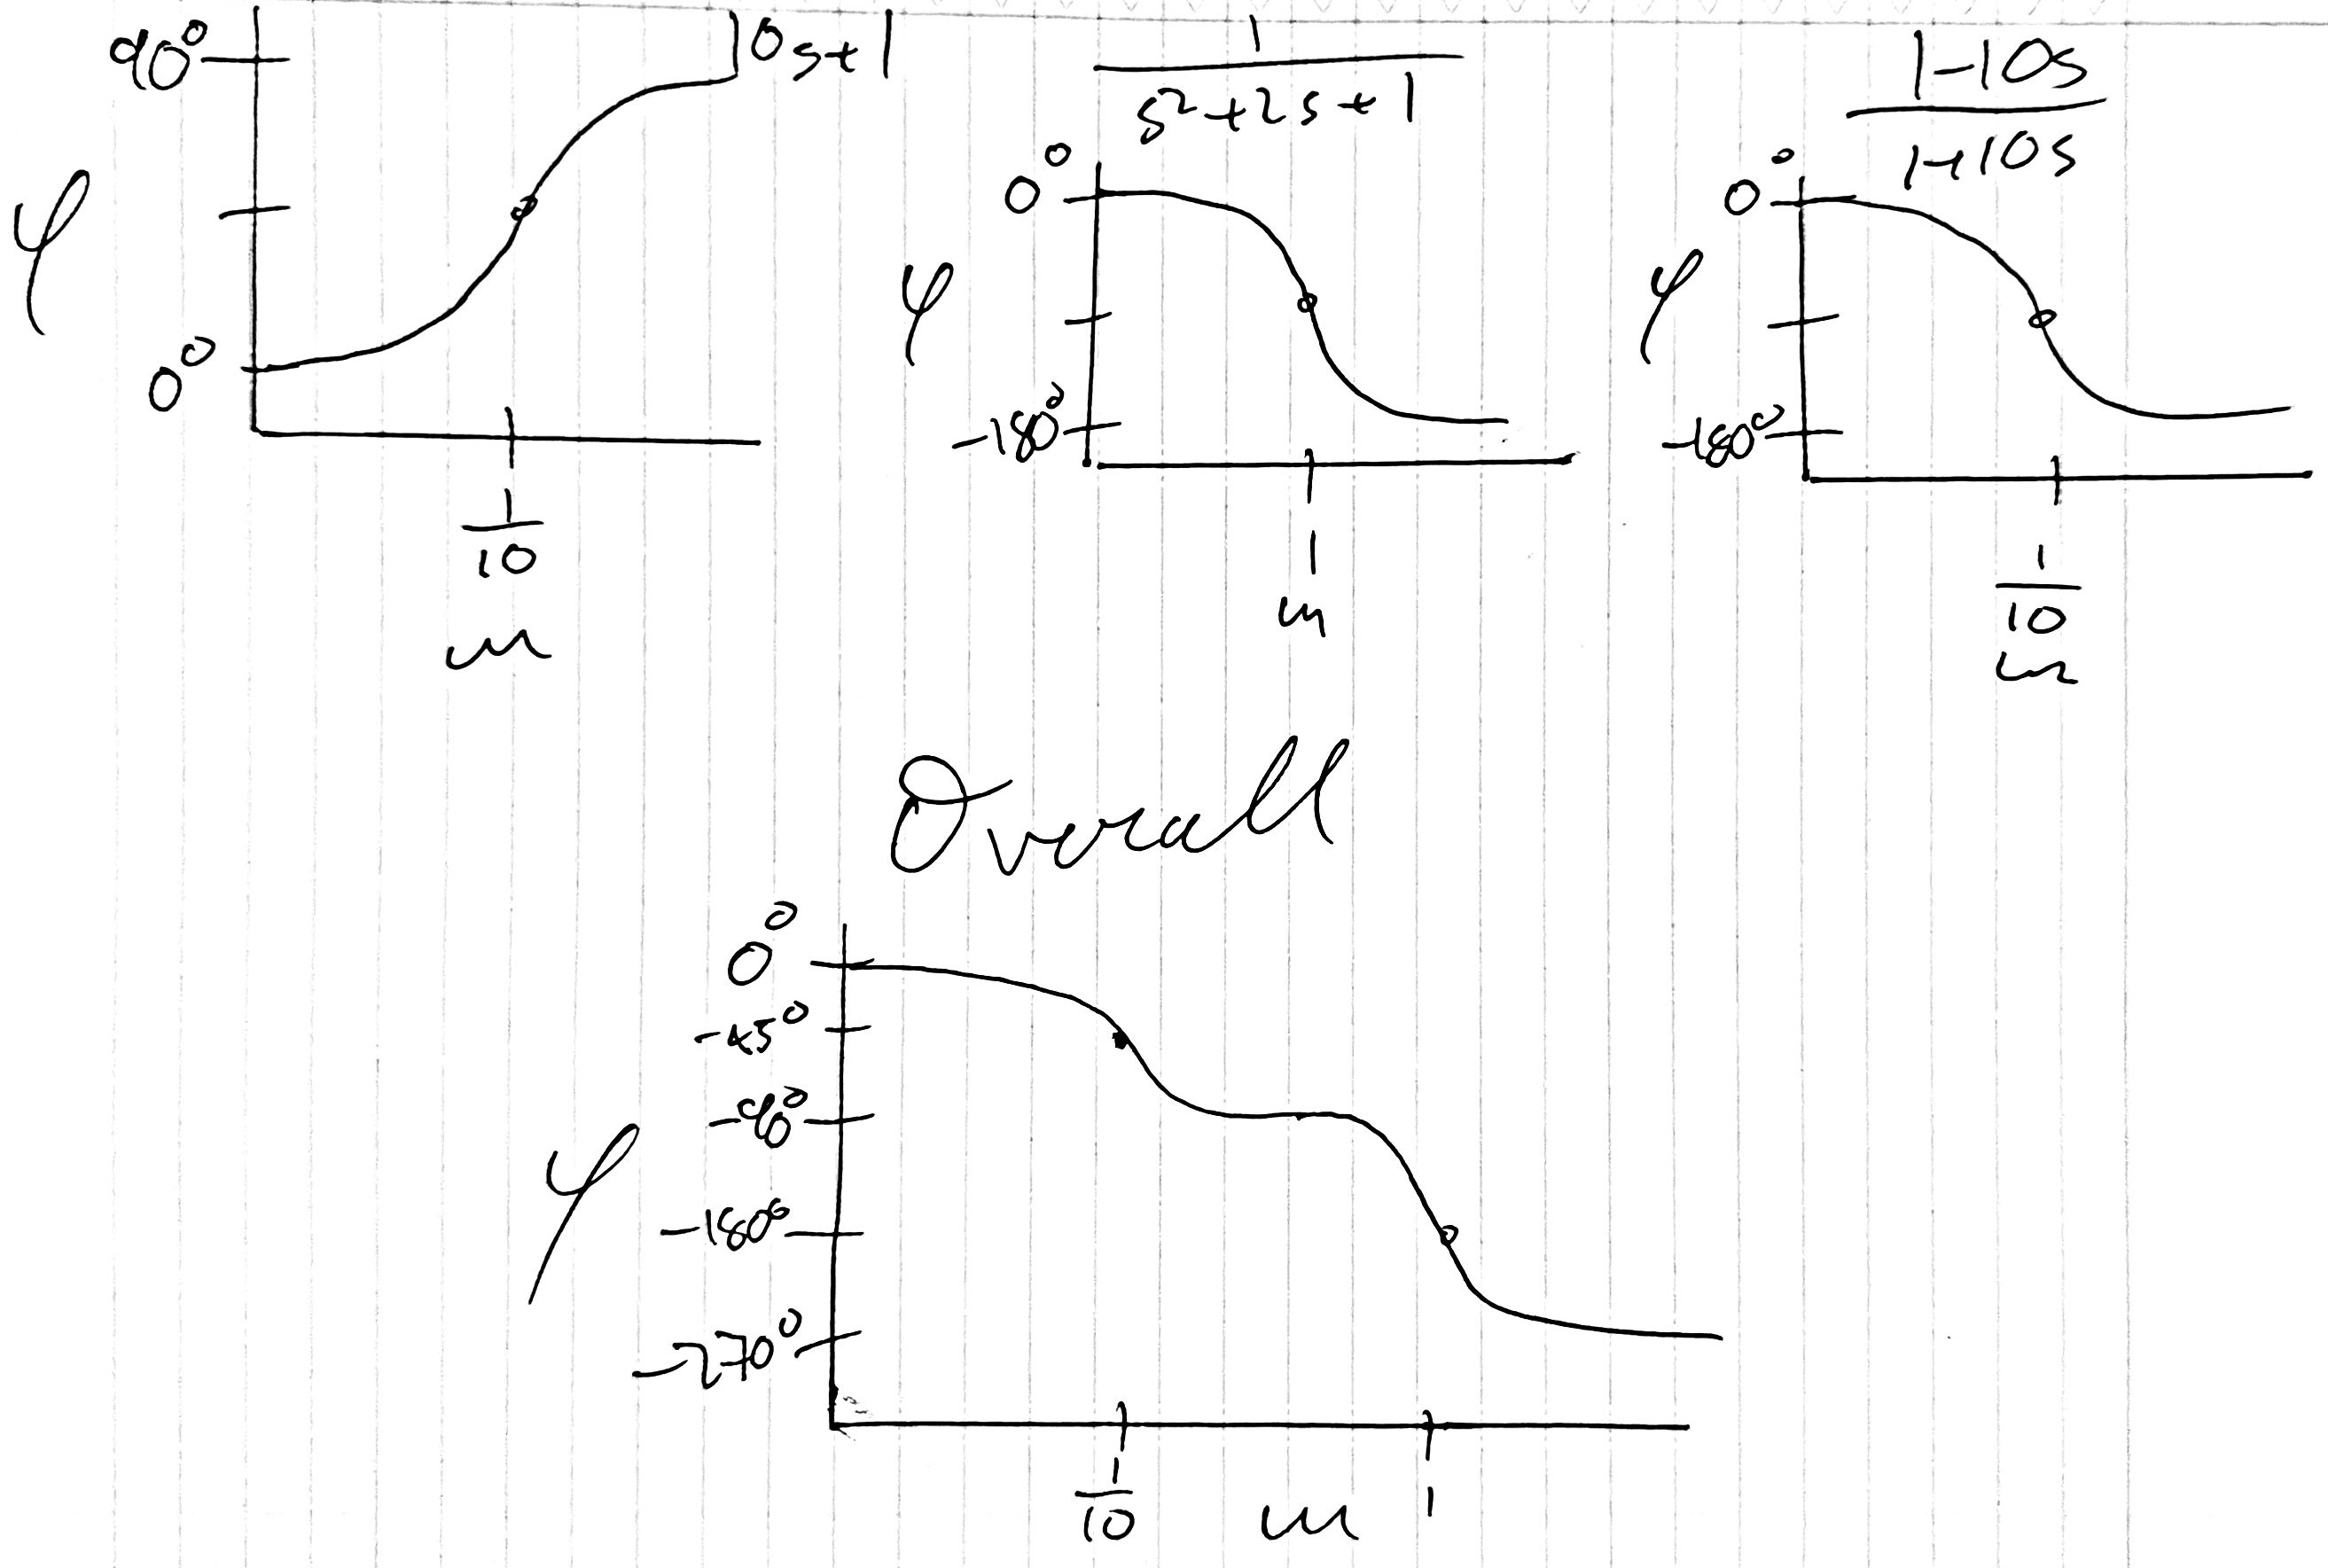
\includegraphics[width=0.8\textwidth]{assets/iii_phase.jpg}
    \end{center}

    Verify:

    \begin{center}
        \includesvg[width=0.8\textwidth]{assets/p3_iii.svg}
    \end{center}

    (iv)

    \begin{align*}
        G(s) &= \frac{1}{\left(s^2+0.1s+1\right)\left(9s^2+0.3s+1\right)} \\
        \intertext{$\frac{1}{\left(s^2+0.1s+1\right)}$ magnitube and phase angle}
        \tau &= 1 \\
        \zeta &= 0.05 \\
        \text{AR} &= \frac{1}{\sqrt{\left(1-\omega^2\right)^2+(0.1\omega)^2}} \\
        \phi &= -\cos^{-1}\left(\frac{1-\omega^2}{\sqrt{\left(1-\omega^2\right)^2+(0.1\omega)^2}}\right) \\
        \intertext{$\frac{1}{\left(9s^2+0.3s+1\right)}$ magnitube and phase angle}
        \tau &= 3 \\
        \zeta &= 0.05 \\
        \text{AR} &= \frac{1}{\sqrt{\left(1-9\omega^2\right)^2+(0.3\omega)^2}} \\
        \phi &= -\cos^{-1}\left(\frac{1-9\omega^2}{\sqrt{\left(1-9\omega^2\right)^2+(0.3\omega)^2}}\right) \\
        \intertext{Overall}
        \text{AR} &= \frac{1}{\sqrt{\left(1-\omega^2\right)^2+(0.1\omega)^2} \cdot \sqrt{\left(1-9\omega^2\right)^2+(0.3\omega)^2}} \\
        \phi &= -\cos^{-1}\left(\frac{1-\omega^2}{\sqrt{\left(1-\omega^2\right)^2+(0.1\omega)^2}}\right) - \cos^{-1}\left(\frac{1-9\omega^2}{\sqrt{\left(1-9\omega^2\right)^2+(0.3\omega)^2}}\right) \\
    \end{align*}

    Sketch bode plots:

    \begin{center}
        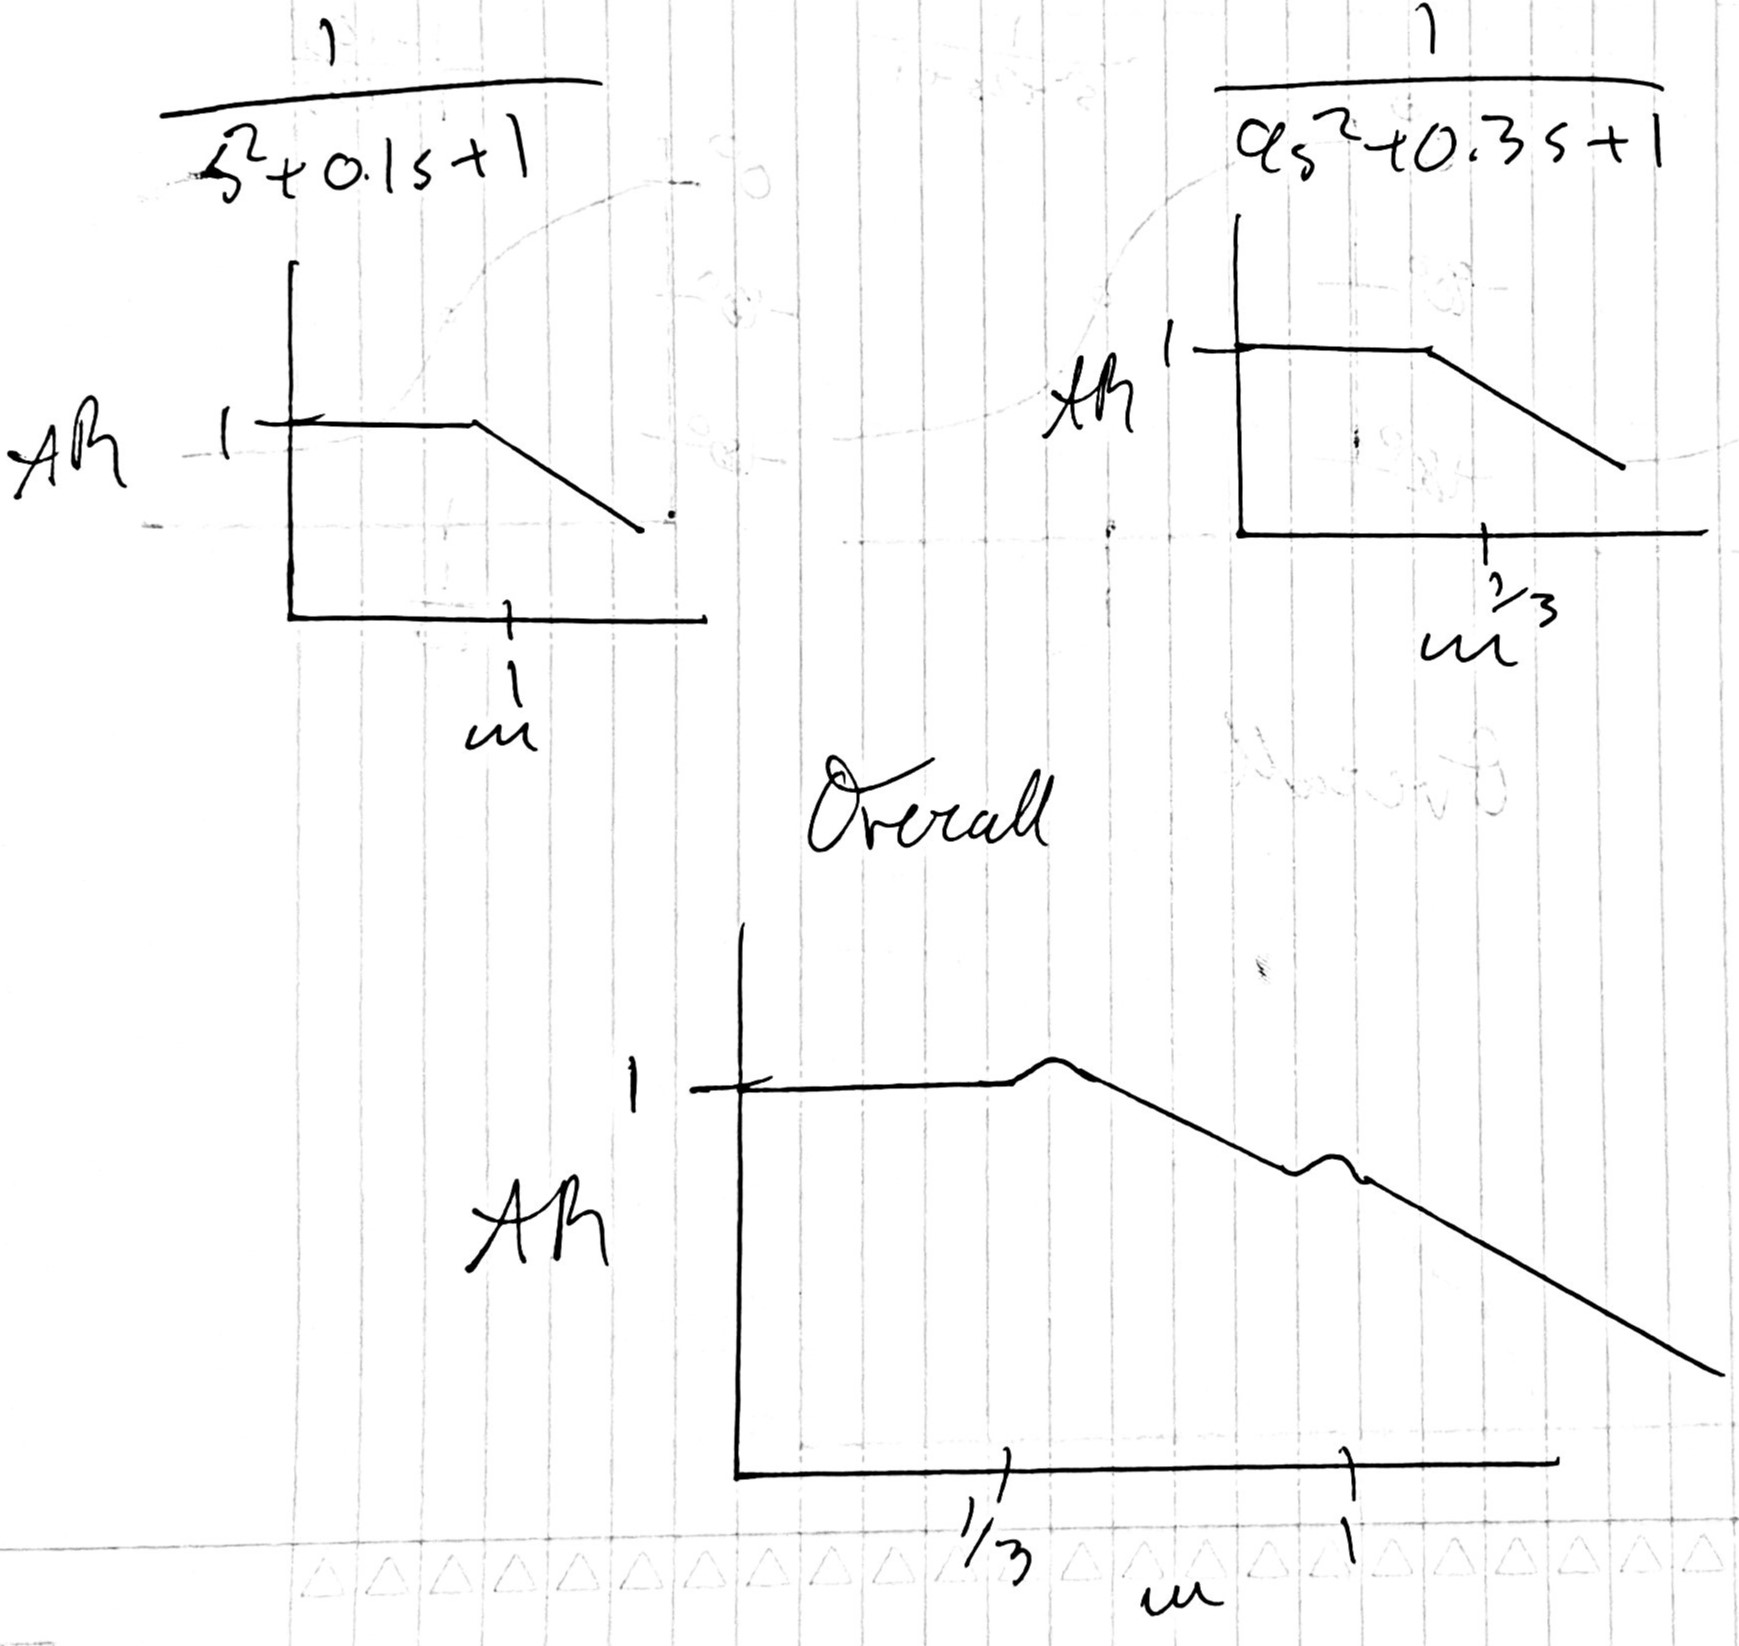
\includegraphics[width=0.8\textwidth]{assets/iv_mag.jpg}
        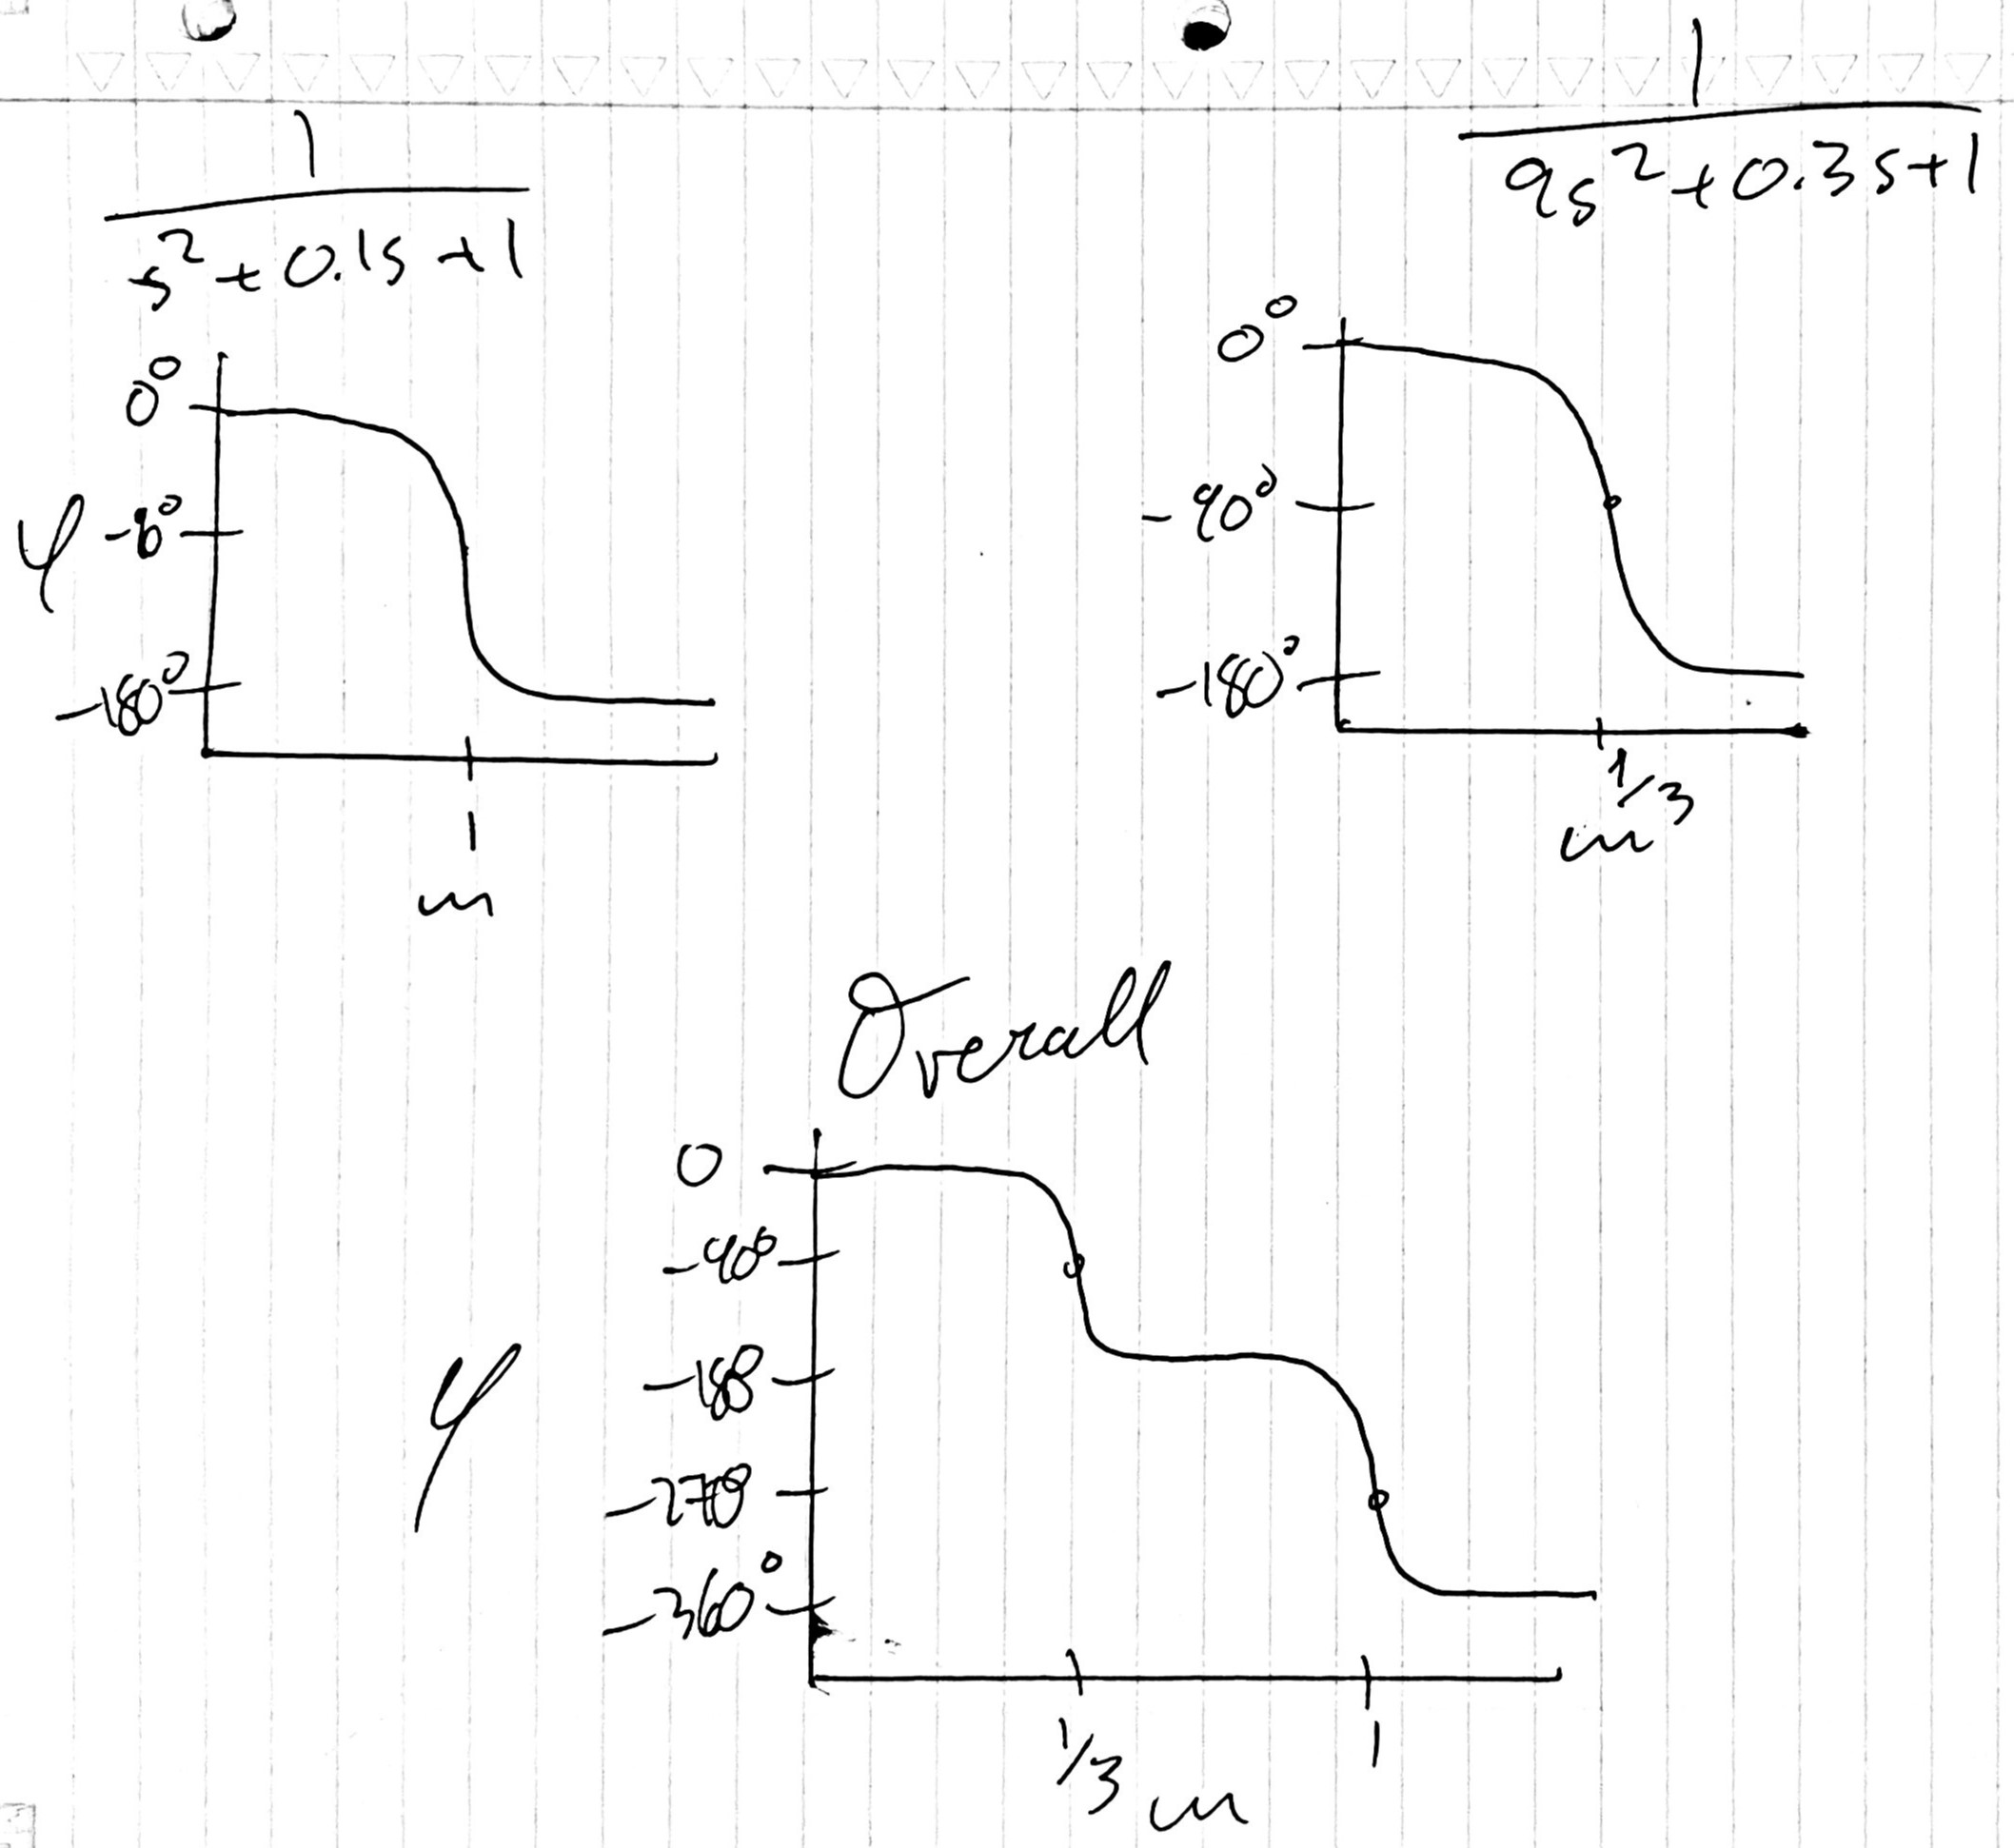
\includegraphics[width=0.8\textwidth]{assets/iv_phase.jpg}
    \end{center}

    Verify:

    \begin{center}
        \includesvg[width=0.8\textwidth]{assets/p3_iv.svg}
    \end{center}

    Code for bode plotting:

\begin{minted}[
framesep=2mm,
baselinestretch=1.2,
bgcolor=LightGray,
fontsize=\footnotesize,
breaklines,
]{python}
import numpy as np
import matplotlib.pyplot as plt
import control

w = np.linspace(1e-3, 1e3, int(1e5))

# i
sys = control.zpk([], [0, -1/0.1, -1/10], 1)
mag, phase, omega = control.bode_plot(sys, omega=w)
plt.show()

# ii
sys = control.zpk([-1/10], [-1, -1], 10)
mag, phase, omega = control.bode_plot(sys, omega=w, wrap_phase=True)
plt.show()

# iii
sys = control.tf([-10, 1], [1, 2, 1])
mag, phase, omega = control.bode_plot(sys, omega=w)
plt.show()

# iv
sys = control.tf([1], [9, 1.2, 10.03, 0.4, 1])
mag, phase, omega = control.bode_plot(sys)
plt.show()
\end{minted}

%%%%%%%%%%%%%%%%%%%%%%%%%%%%%%%%%%%%%%%%%%%%%%%%%%%%%%%%%%%%%%%%%%%%%%%%
% Problem 4 %%%%%%%%%%%%%%%%%%%%%%%%%%%%%%%%%%%%%%%%%%%%%%%%%%%%%%%%%%%%
%%%%%%%%%%%%%%%%%%%%%%%%%%%%%%%%%%%%%%%%%%%%%%%%%%%%%%%%%%%%%%%%%%%%%%%%
\newpage
    \item Problem 9.10

    There are inflection points at $\omega = 0.1$ and $\omega = 10$. These values correspond to $T$ and $\tau$. Between $\omega = 0.1$ and $\omega = 10$ the integrator and lead need to be active so that the AR plot is flat in that frequency range. Thus $\boxed{T=10}$ and $\boxed{\tau=0.1}$.

    Simulating each transfer function, a numerator of [-10, 1] and a denominator of [0.1, 1, 0] produce the correct shape of the phase plot. There has to be an all pass because the phase angle is constantly decreasing. Having a lead with a positive $\tau$ would result in a peak. The numerator has to be [-10, 1] becasue the shape of the phase plot suggests that there needs to be an all pass active.

    At $\omega = 0.001$ the AR is approximately 1000. That makes the the static gain 1. So, $\boxed{k=1}$.

    If the transfer funtion has a second order lead then the AR would decrease much faster after $\omega = 10$.

    The correct transfer function is (d)
    \[
        G_4(s) = k \frac{-Ts + 1}{s (\tau s + 1)}  
    \]

    \[
        G_4(s) = \frac{-10s + 1}{s (0.1 s + 1)}  
    \]

    Recreation of bode plots with estimated parameters:

    \begin{center}
        \includesvg[width=0.8\textwidth]{assets/p4.svg}
    \end{center}

    The recereated bode plot is the same as the bode diagram given in the problem statement.

    Problem 4 code:

\inputminted[
framesep=2mm,
baselinestretch=1.2,
bgcolor=LightGray,
fontsize=\footnotesize,
breaklines,
]{python}{p4.py}
    
\end{enumerate}
\end{document}